%\newpage
\section{任务介绍}

\subsection{建模对象描述}

所选定建模对象的系统特性将从\textbf{集合性、相关性、环境适应性}三个方面来分析。

\subsubsection{集合性}

该系统由机械主体模块和电驱动模块组成,二者缺一不可。 在创建物理设备建模仿真时,主要任务是实现集成控制驱动系统和执行器动态的模型,以便将仿真软件工具集成到模过程中。 

所谓执行机构在这里指的是机械主体模块,主要是由底盘与轮系。所谓控制驱动系统是指为机械系统提供动力的部分,这里主要指电驱动模块(如图~\ref{fig:PW_parts})。电驱动模块由电源,电机,齿轮等部分组成,电源供应整体电机及驱动的能量,电机转动先经过齿轮减速器减速增扭,最终传递到驱动轮轮系上,从而实现整体电动轮椅的功能。

\subsubsection{相关性}

就整体电动轮椅系统而言,子系统相互依存、相互制约、相互作用形成了相互关联的整体。

机械主体模块和电驱动模块间的联系是通过电机输出轴和驱动轮具有共同的位置和速度借助联轴器来实现的。通过电机轴的运动,实现驱动轮的转动。研究对象的机械主体和电驱动模块之间相互关联的变量是轴系转动的角速度。通过两者相互固定实现,势和流的传递。

%%%%%%%%%%%%%%%%%
\begin{figure*}[!h]
	\centering
	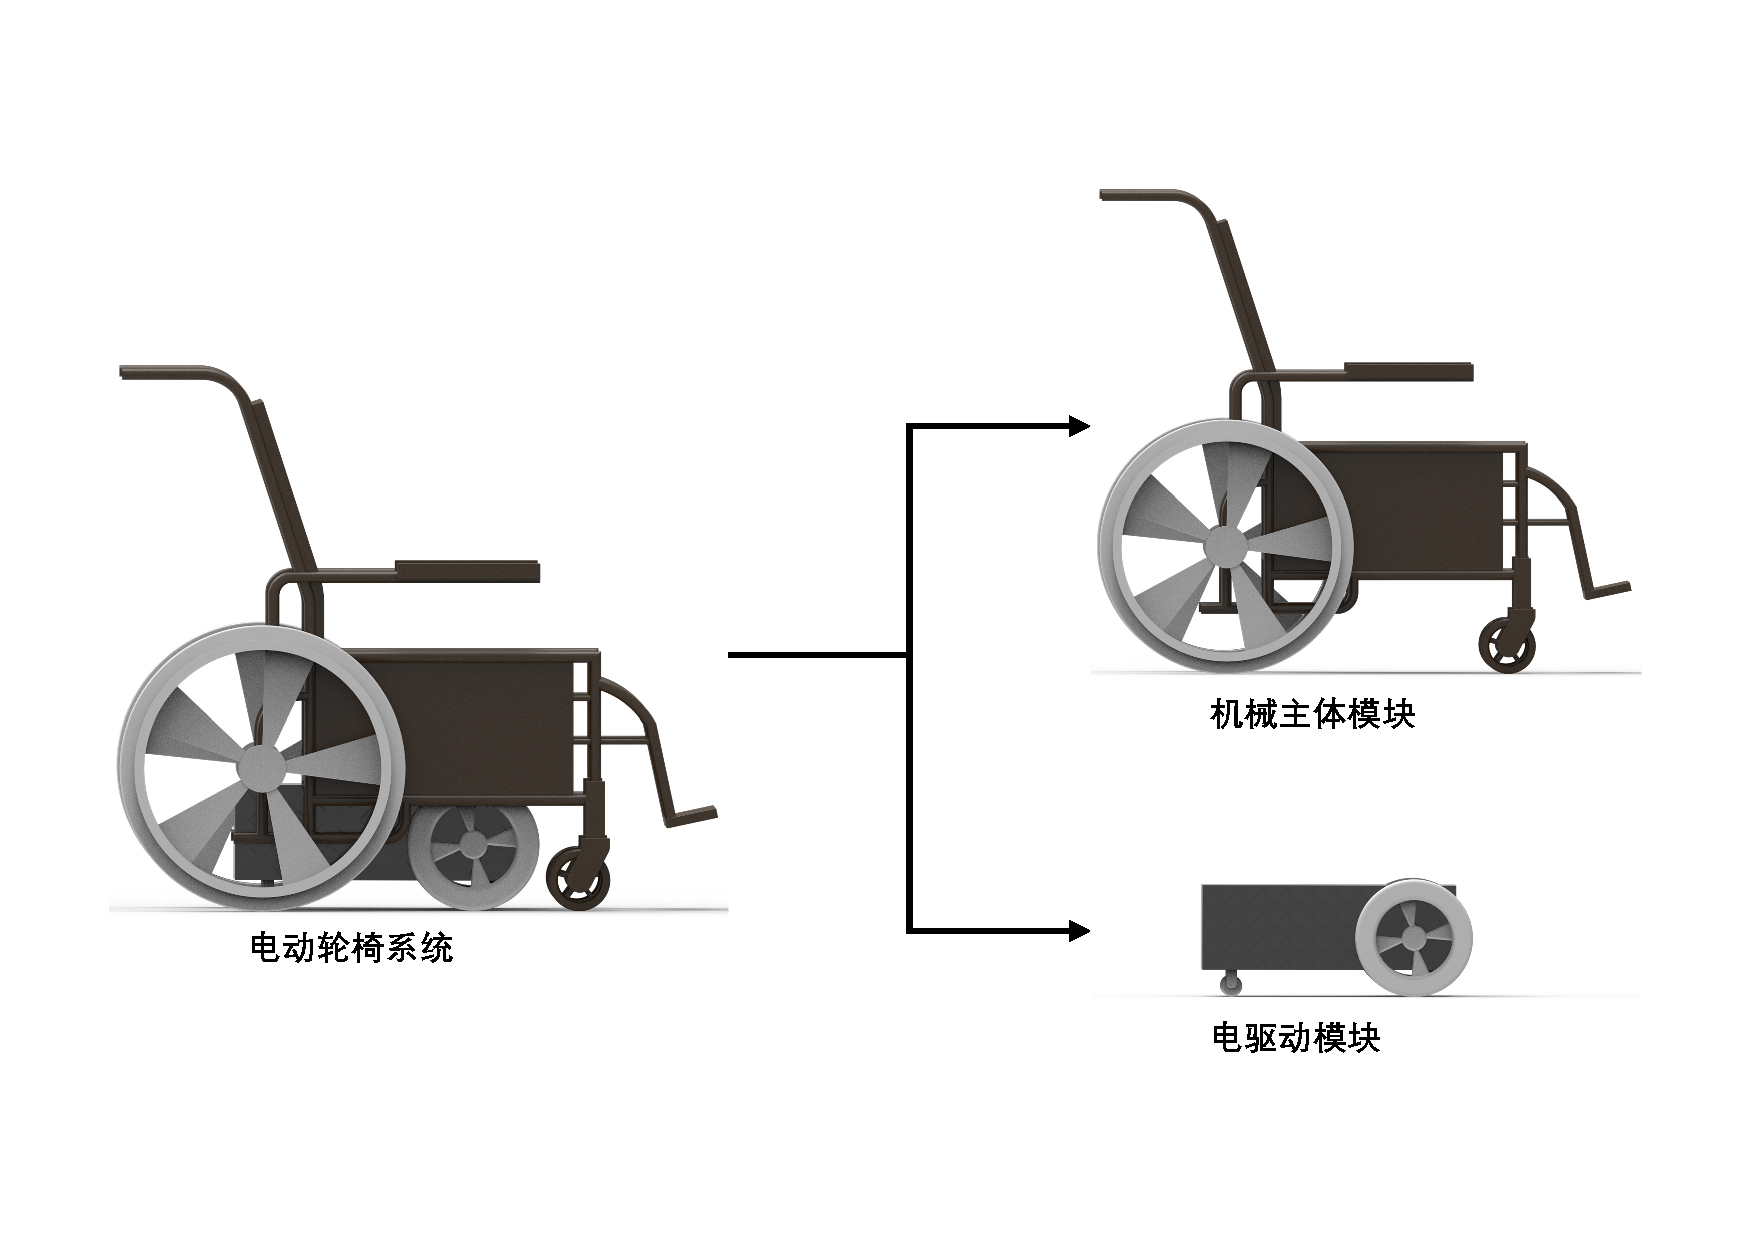
\includegraphics[width=0.96\textwidth]{fig/PW_parts.pdf}
	\caption{选取电动轮椅组成部分。}\label{fig:PW_parts}
\end{figure*}
%%%%%%%%%%%%%%%%%

\subsubsection{环境适应性}

传动的手推轮椅,结构简单,给行动不便人士以更大活动空间。但是在日常生活使用中,一般还是需要额外的人力用于前后左右前进与旋转运动。而机电模块的加入,将有效提高该设备的智能化程度,我们同时可以将相关移动机器人的控制分析理论应用其中。

在移动机器人中,主要分为轮式,履带式,足式等系统,通过机械与机电模块相结合,能够非常有效地处理平坦且结构良好的固体表面,从而满足行动不便人士的需求。

\subsection{建模问题提取}

可以将对象的工况分为两种情况:

\begin{enumerate}
	\item 在平坦路面上条件下,由人产生推力使轮椅向前运动。
	在该条件下,系统底部受到的速度输入较小且较不稳定。主要考虑以下几个参数:
	\begin{itemize}
		\item 车轮转动惯量,转动惯量;
		
		\item 车轮辐条刚度:存在于从车轮中心到地面由于充气轮胎所带来的弹簧/阻尼;
		
		\item 摩擦损失:存在于后充气轮和前脚轮与地面之间的阻力;
		
		\item 质量:包括椅子的重量和使用者的假定质量。该点位于重心处,获得系统平均质量。在降低模型的复杂性时,假设重心与后轮轴线中心重合。
	\end{itemize}
	
	\item 在平坦路面上条件下,由机电驱动模块产生使轮椅向前运动的动力。
	在该条件下,系统底部受到的速度输入较大且较稳定。主要考虑以下几个参数:
	\begin{itemize}
		\item 直流电动机的基本原理(包括电感,输出扭矩等)和基本性质(包括质量,电压等)。
		
		\item 传动部件的刚度,质量以及机械损失。
		
		\item 电动轮的转动惯量。
	\end{itemize}
	
\end{enumerate}

\subsection{模型假设与标记}

\subsubsection{模型假设}

针对上述工况,结合简化模型的角度出发,做出如下假设:

\begin{itemize}
	
	\item 假设机械各部分零件为刚体;
	
	\item 假设刚体质心位于几何中心;
	
	\item 忽略铰接点连接处的摩擦;
	
	\item 忽略电驱动系统工作产热带来的参数变化。
	
\end{itemize}

\subsubsection{模型标记}

表 \ref{tab:param} 列出本模型的相关参数及其数学标记。主要分为分为整体系统参数,手推轮椅主体,机电驱动模块以及手推控制输入部分的参数,如下所示:

\begin{table}[H]
\caption{系统主要参数及其数学标记}\label{tab:param}
\begin{longtable}{l|l}
	\toprule
	\textbf{数学标记} & \textbf{系统参数}\\
	\midrule
	\endhead
	\multicolumn{2}{l}{\textbf{系统整体参数}} \\ % {占用行数} {文字居左中右} {内容}
	\midrule
	$ M $ & 总体质量\\
	$ J $ & 总体转动惯量\\
	$ V_{\rm{CG}} $ & 质心速度\\
	$ w_{\rm{CG}} $ & 质心转速\\
	$ P_{\rm{CG}} $ & 系统动量变化率\\
	$ P_{\theta} $ & 系统角动量变化率\\
	\midrule
	\multicolumn{2}{l}{\textbf{手推轮椅主体}} \\
	\midrule
	MSE:$\tau$ & 后轮推进扭矩 \\
	$ J w $ & 后轮转动惯量\\
	$ M_t $ & 系统质量\\
	$ J t $ & 系统转动惯量\\
	$ R_g $ & 轮胎与地面摩擦系数\\
	$ C_w $ & 轮辐弹性系数\\
	$ R_w $ & 轮辐阻尼\\
	$ r $ & 后轮半径\\
	$ L_w $ & 轮椅宽度\\
	\midrule
	\multicolumn{2}{l}{\textbf{机电驱动模块}} \\
	\midrule
	$ I_e $ & 电机电感\\
	$ R_e $ & 电机内阻\\
	$ J_r $ & 转子转动惯量\\
	$ R_b $ & 电机轴承阻尼\\
	$ M_d $ & 机电驱动模块质量\\
	$ J_d $ & 机电驱动模块转动惯量\\
	$ L_d $ & 模块宽度\\
	$ C_s $ & 电机输出转矩\\
	$ R_s $ & 电机输出轴阻尼\\
	$ k_1 $ & 电机扭矩系数\\ % 简化了k8
	$ k_2 $ & 齿轮系数比\\ % 简化了k7
	$ k_3 $ & 电动车轮半径 \\ % 简化了k6
	MSe:L & 输入控制电压\\
	\midrule
	\multicolumn{2}{l}{\textbf{手推控制输入部分}}\\
	\midrule
	$ J $ & 手动轮转动惯量\\
	$ k_4 $ & 手动轮半径\\ % 简化了k10
	\bottomrule
\end{longtable}
\end{table}